\section{Performance Evaluation}
\label{Testing}

After implementing the aforementioned tasks, we run an experiment in order to test the average performance of the MAP and MPE algorithm with three different elimination order algorithms; the random order, the min-order and min-fill heuristics described in Section \ref{BNReasoner}. The metrics used to evaluate the results are the following:
\begin{itemize}
    \item Run time
    \item Number of nodes
    \item Tracked degrees throughout the execution
\end{itemize}
The experiment has been run ten times per heuristic for each algorithm, and the average of those runs is presented in the later plots for each metric.

\subsection{Experiment Preparation}
We created a script that generates different Bayesian networks to implement the experiment. Each implemented network has two root nodes and a minimum number of five variables, while every child has a minimum of one parent and a maximum of three. During the experiment, each generated network grew by ten nodes each time. A total number of five networks was created and used for this experiment. 
Regarding the queries, we chose to have the same ratio of given evidence and map variables in the five Bayesian Networks mentioned above, aiming to compare the performance of the implementation independently of the given parameters. For both queries, the ratio of given evidence equals $2.5$, i.g a five-node BN corresponds to $5/2.5$ evidence, while a fifteen-nodes BN to six given evidence. The same logic stands for the MAP variables ratio used in the MAP queries, which equals $2$. The variables selected as evidence cannot be chosen as MAP variables.

\subsection{Results}
As shown in Figure \ref{fig:time_nodes}, the two heuristics generally outperform the random order in both MPE and MAP queries. The first graph shows that all three elimination order functions run approximately the same time between five and fifteen nodes. However, from twenty-five nodes onwards, the two heuristics perform roughly the same as before, while the random order grows exponentially.\\
Regarding the second graph of the figure, the run time for a MAP query is illustrated. As can be seen, the number of nodes and the run time increase accordingly, with the random order requiring the most time once again. The difference is not as noticeable as in the previous graph, but it is still significant.

\intextsep
\begin{figure}[H]
    \centering
    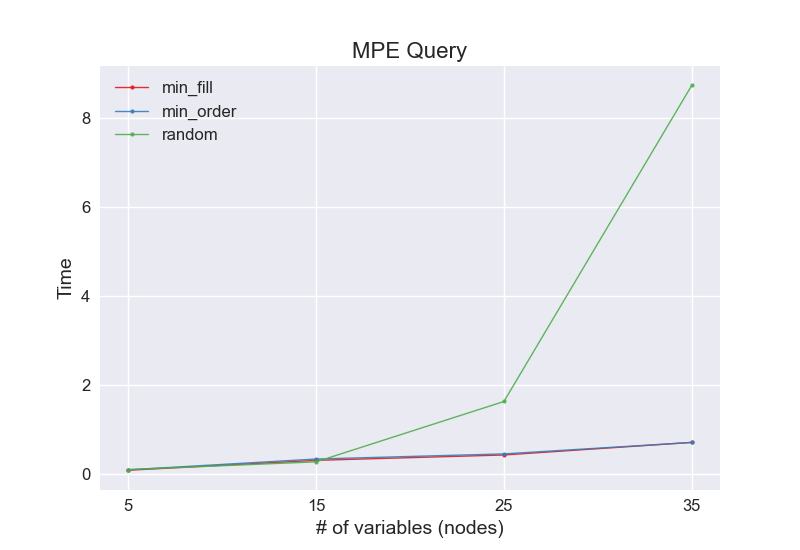
\includegraphics[width=0.45\textwidth]{Assets/mpe_query.png}
    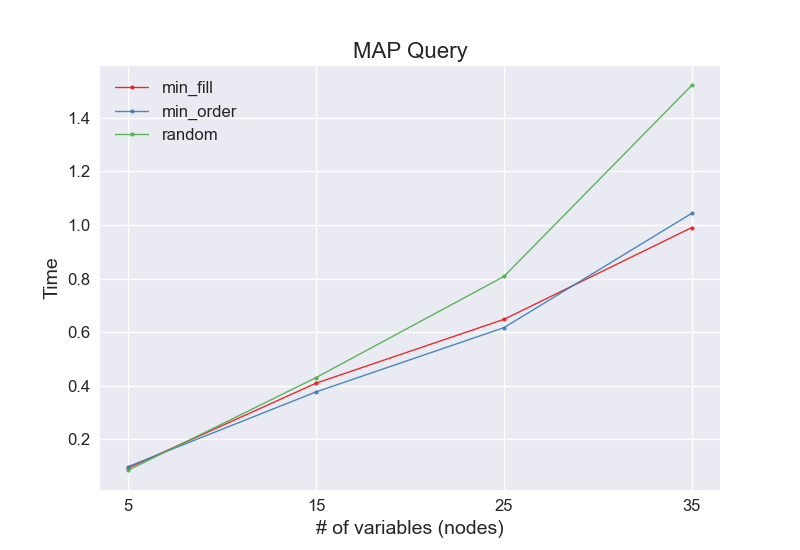
\includegraphics[width=0.45\textwidth]{Assets/map_query.png}
    \caption{Number of nodes vs. Time}
    \label{fig:time_nodes}
\end{figure}\\



To evaluate further the different orderings,  we tracked the degrees of each order during the execution of the queries. In other words, every time an elimination occurred in the algorithm, we counted the number of variables included in the newly created factor. This number corresponds to the width of the used order π and is a way to measure the order quality. In the figures \ref{fig:mpe_histograms} and \ref{fig:map_histograms}, three different histograms are illustrated per query, and each histogram represents how many times each degree occurred in the five, twenty-five and forty-five BNs, respectively.

The different degrees tracked in the MPE Queries are shown in Figure \ref{fig:mpe_histograms}. Based on the graphs, the degrees occurred using the heuristics overlap in all tested BNs independently of the variable size and fluctuate in a smaller scale than random order. The histogram correlates perfectly with the line plot in Figure \ref{fig:time_nodes}.

\intextsep
\begin{figure}[H]%
    \centering
    \subfloat[\centering a ]{{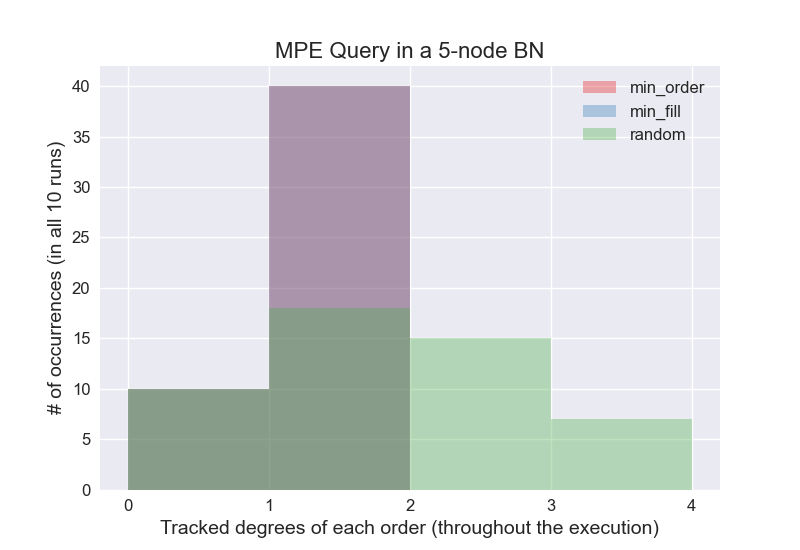
\includegraphics[width=5.2cm]{Assets/mpe-hist.png} }}%
    \qquad
    \subfloat[\centering b ]{{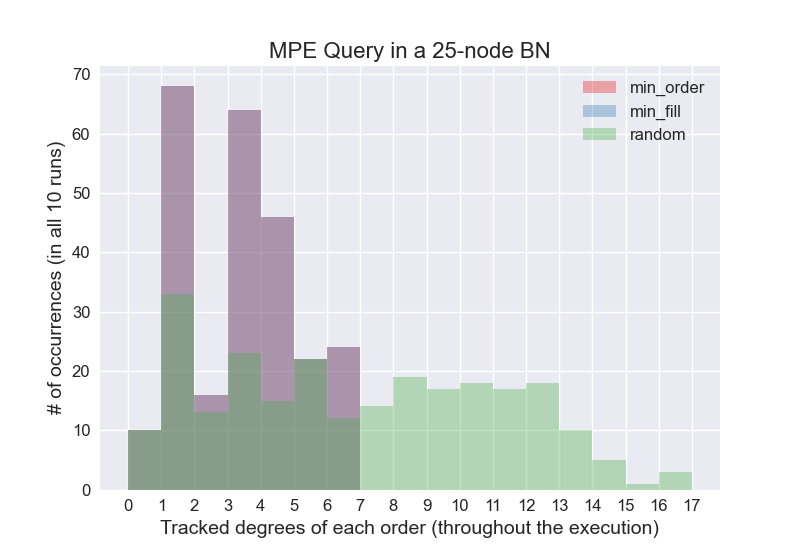
\includegraphics[width=5.2cm]{Assets/mpe-hist-25nodes.png} }}%
    \qquad
    \subfloat[\centering c ]{{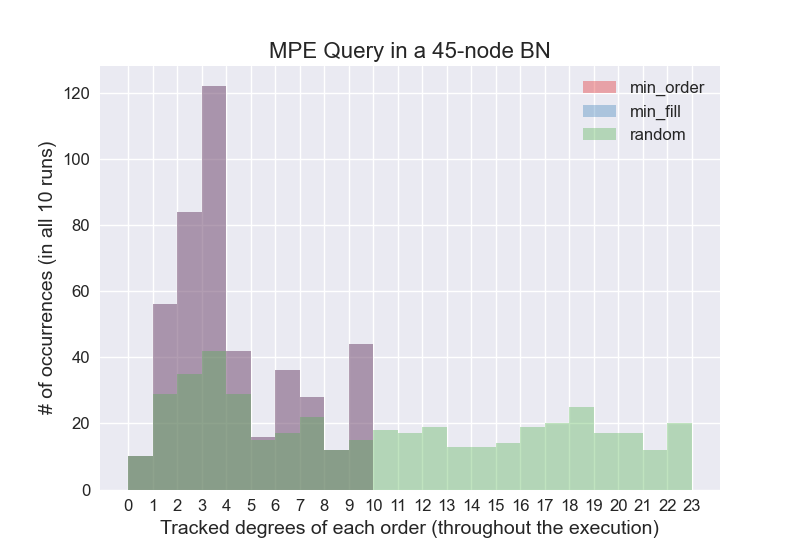
\includegraphics[width=5.2cm]{Assets/mpe-hist-45nodes.png} }}%
    \qquad
    \caption{MPE Queries}%
    \label{fig:mpe_histograms}%
\end{figure}

On the other hand, in Figure \ref{fig:map_histograms}, the degrees of the two heuristics do not match for more than twenty-five node BNs when executing the MAP queries. Nevertheless, the width fluctuates in a similar scale with min-fill to perform slightly better than the min-order heuristic. Regarding the random orderings, the width reaches higher numbers than the other two methods.

\intextsep
\begin{figure}[H]%
    \centering
    \subfloat[\centering a ]{{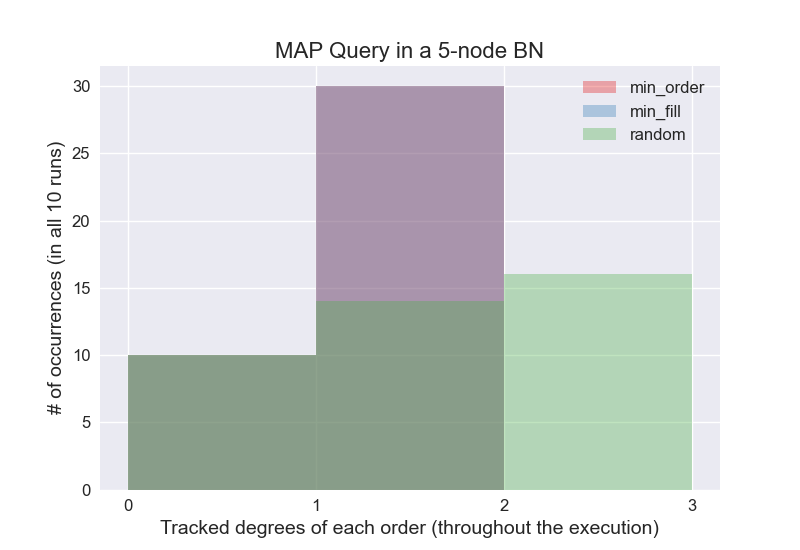
\includegraphics[width=5.2cm]{Assets/map-hist.png} }}%
    \qquad
    \subfloat[\centering b ]{{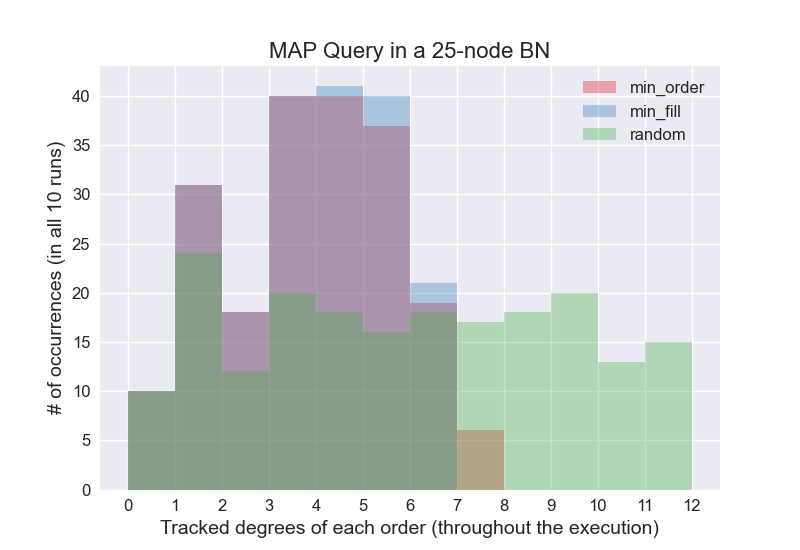
\includegraphics[width=5.2cm]{Assets/map-hist-25nodes.png} }}%
    \qquad
    \subfloat[\centering c ]{{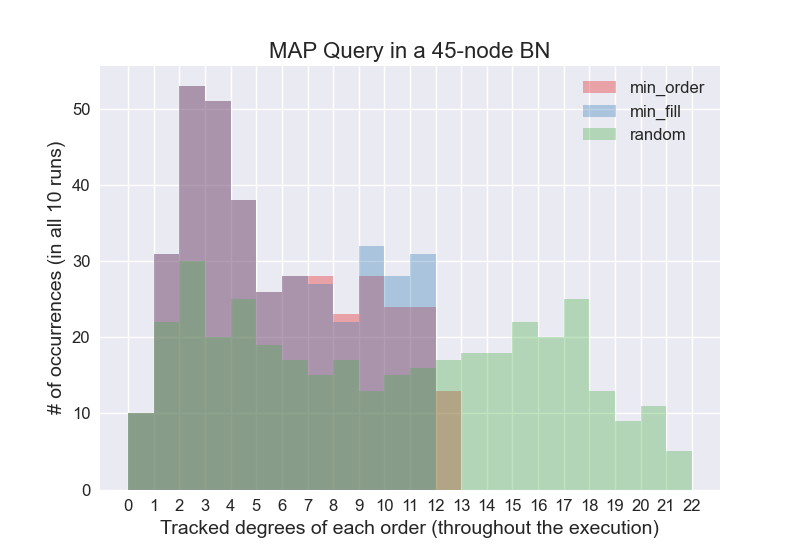
\includegraphics[width=5.2cm]{Assets/map-hist-45nodes.png} }}%
    \qquad
    \caption{MAP Queries }%
    \label{fig:map_histograms}%
\end{figure}
\\\\
In general, the experiment results highlight the superiority of the implemented heuristics over randomness and the importance of the elimination order. The computational complexity decreases in correlation to the quality of the order. 
